\chapter{About the technology stack}
\label{cha:techstack}

Before describing the entire project, we need to know what we are talking about. In particular, there are the softwares or libraries strongly used in the project:  
\begin{itemize}
    \item Docker
    \item ROS2
    \item Gazebo
    \item Navigation stack, nav2
    \end{itemize}

\section{\acrshort{ros}2}

\begin{wrapfigure}{l}{0.2\textwidth}
    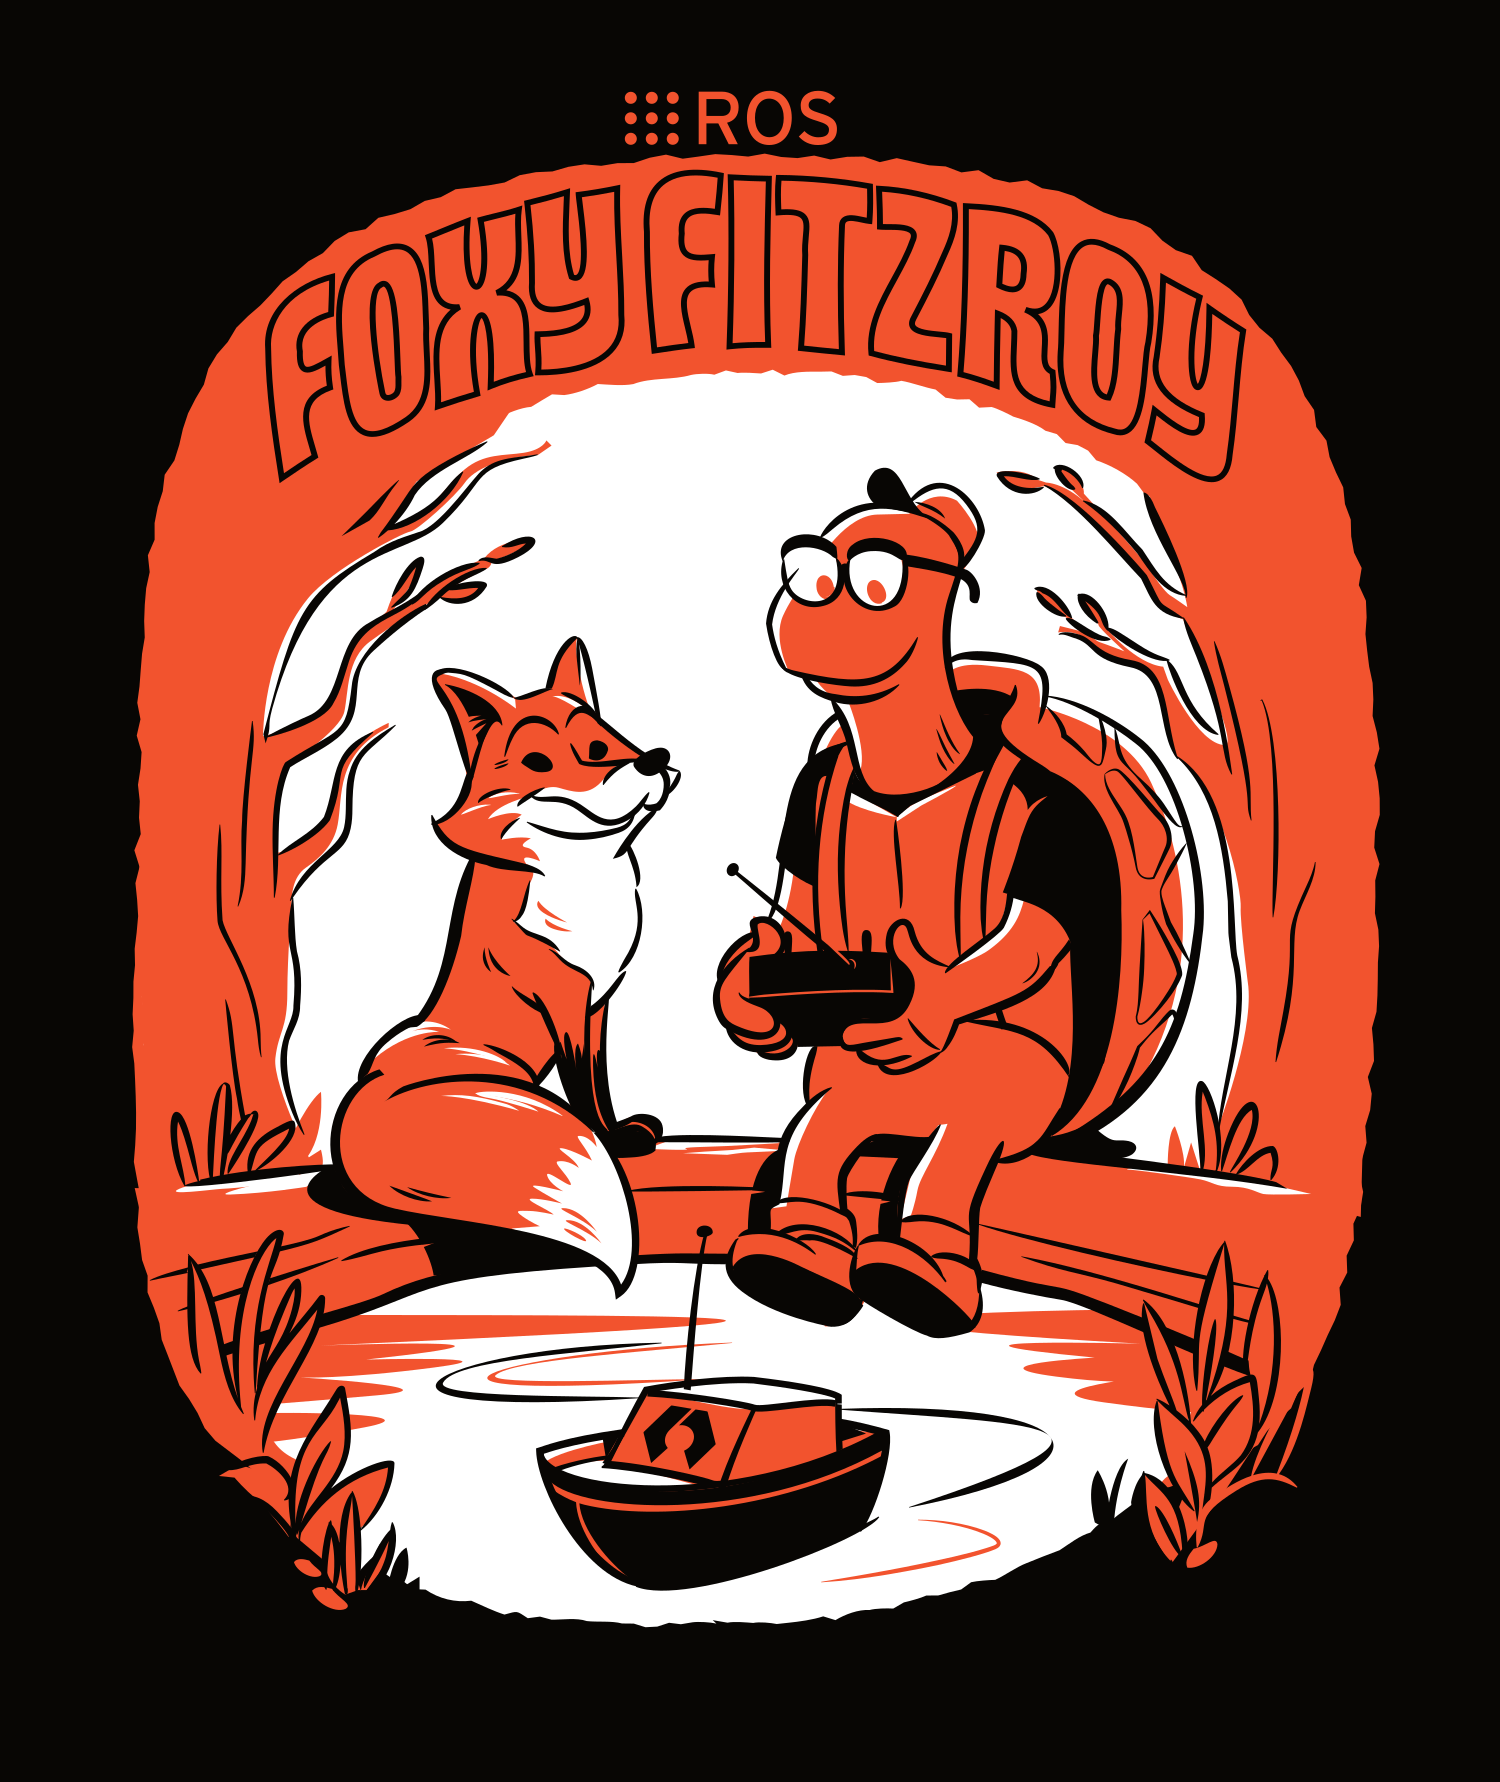
\includegraphics[width=0.2\textwidth]{images/foxy}
\end{wrapfigure}

\textit{\acrshort{ros}2, which stands for Robot Operative System 2, is a set of software libraries and tools for building robot applications.}\cite{ros2desc} On it, every process is a node and each node has the possibility to talk to other ones thanks to some channel of communications called topics using the publish/subscribe model.

This version of \acrshort{ros}2, called \textbf{Foxy}, was used because it is possible to integrate the \textit{plansys2} libraries used for planning.

Thanks to \Acrshort{ros} \textit{hardware abstraction, low-level device control, implementation of commonly-used functionality, message-passing between processes, and package management}\cite{ros2help}, the developer can ignore specific hardware details and software implementations and focus only on the application itself. 

This means that executing a \acrshort{ros} node on your own computer is the same of executing it on a robot, as long as you are using the same operative system (only \textbf{Ubuntu 20.04}) and the same external devices, if you are not simulating them.

\section{Gazebo}
\label{sec:gazebo} % add more info about gazebo (?)

\begin{wrapfigure}{r}{0.3\textwidth}
    
\includegraphics[width=0.3\textwidth]{images/gazebo}
\end{wrapfigure}

Here comes the simulation part, because thanks to Gazebo-ROS integration it is possible, with some additional libraries, to simulate external devices. It is not limited to this, because it gives you a sandbox you could set up as the real environment you want to simulate.

In this way, you don't need to have the real robot next to you, you can just use a virtual one: it's very useful in the case you want to change some algorithms or parameters, and you need to test them even if you are on the opposite side of the world.

% includere il fatto che l'ho fatto per questo motivo la parte di simulazione?

\section{\acrfull{rviz}}

\begin{wrapfigure}{l}{0.25\textwidth}
    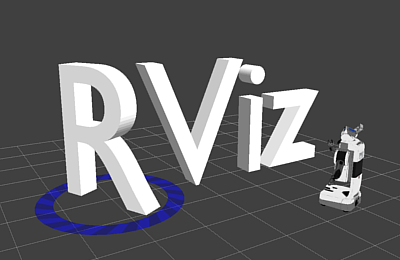
\includegraphics[width=0.25\textwidth]{images/rviz}
\end{wrapfigure}

\Acrshort{rviz}, is a visualization tool for ROS: in this way, you are able to visualize the sensors, the robots, the environment, and also the algorithms; in general, you can see the actual state of your \acrshort{ros} system. % aggiungere roba (?)

\section{\acrfull{nav2}}

The Navigation Stack is a collection of packages of \acrshort{ros}2 which provides useful tools helping you with the navigation of your robot: path planning, localization, and so on. You can use it by passing your desired configurations in a YAML file which will be used when you launch the navigation stack: basically, you specify what nodes you want to use and the parameters you want to set, and everything is done for you. (?)
These packages were used as a base to everything else, so in this way I don't need to worry about the navigation algorithms, since my goal is to develop a system to move around ground robots where indicated.

\begin{figure}[h]
    % \noindent\makebox[0.9\textwidth]{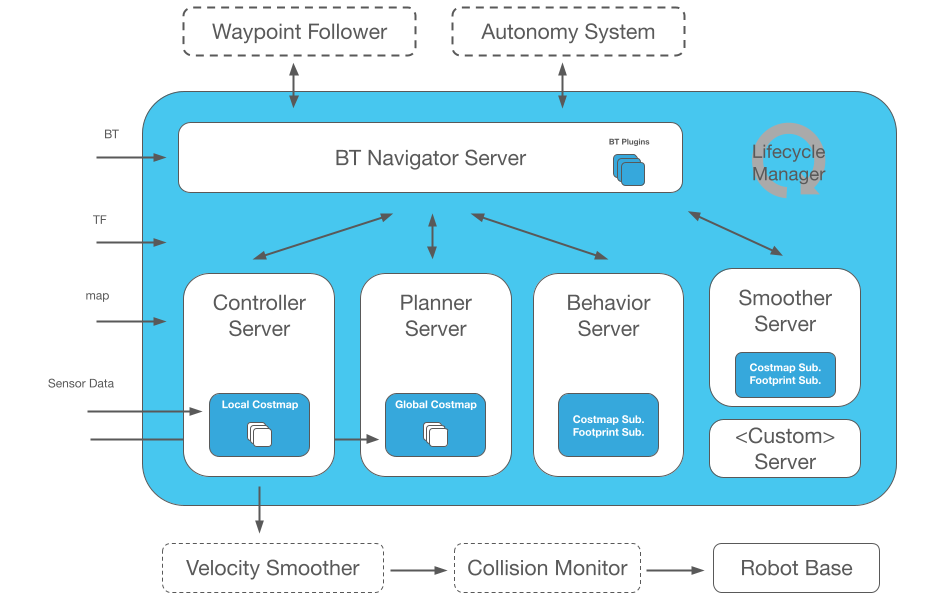
\includegraphics[width=0.9\paperwidth]{images/nav2_architecture}}
    \centering
    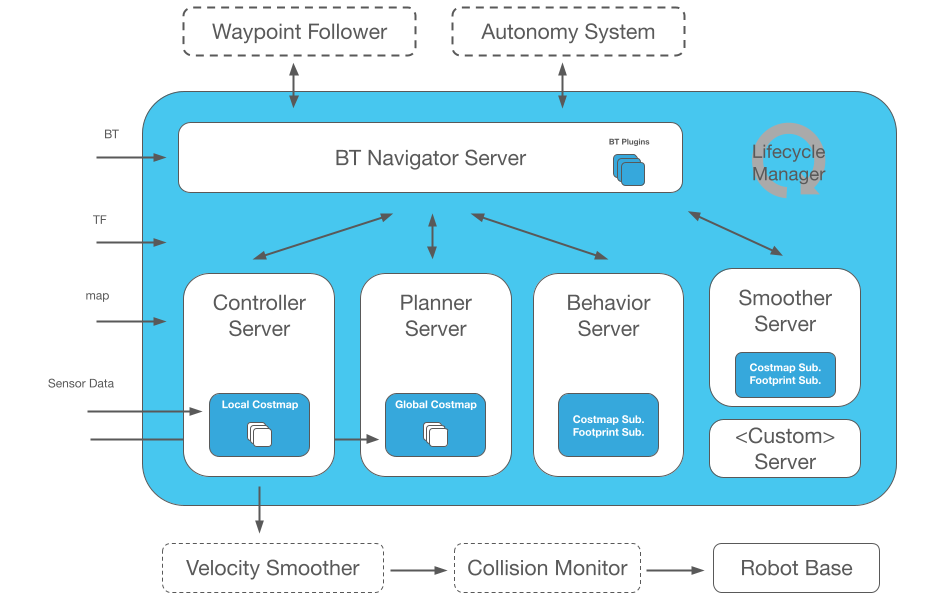
\includegraphics[width=0.8\textwidth]{images/nav2_architecture}
    \caption{Navigation architecture}
  
  \end{figure}

\section{Docker}

\setlength\intextsep{0pt}
  
\begin{wrapfigure}[3]{r}{0.15\textwidth}
    
\includegraphics[width=0.15\textwidth]{images/docker}
\end{wrapfigure}
  
Docker is a platform that let you separate your application using an isolated environment called container. It gives you also the possibility to run multiple containers at the same time. As it was originally designed, Docker was used in this project for the following reasons: % basta? (?)
  
\begin{itemize}
    \item \textbf{separate} this project workspace from all the other ones, to \textbf{avoid conflicts}
    \item keep the workspace \textbf{equal} for \textbf{every device} (real robot or simply a computer)
    \item permit development on any device \textbf{not running} necessarily \textbf{Ubuntu 20.04} (required from \acrshort{ros}2) as its OS
\end{itemize}  
  
Inside a Dockerfile, a file containing instructions on how to build an image\footnote{It is used as a starting point when launching a container} with your own configurations, were typed all the commands required to install the missing packages from the base image already containing basic \acrshort{ros}1 and \acrshort{ros}2 packages \cite{dockerimage}. The complete Dockerfile could be found in \autoref{cha:dockerfile}.